\titleformat{\section}{\normalfont\normalsize\bfseries\raggedright}{Appendix \thesection.}{0.5em}{}
\section{Supplementary data and parameters}
\label{app:data}
\appendixnumbering

This appendix lists the parameters with their sources, compares the two workload traces and shows the case-day time
series and the coincidence of the drivers. Parameters are tagged as taken from a cited source [S], derived from public
data [D] or assumed [A]; every assumed value is varied in the sensitivity studies of \secref{sec:res-sens}.

\begin{table}[!htb]
\caption{Workload traces: PAI (2020) and Acme Seren (2023).}
\label{tab:acme}
\centering\footnotesize
\setlength{\tabcolsep}{3pt}
\begin{tabular}{@{}lcc@{}}
\toprule
 & PAI 2020 & Acme Seren 2023\\
\midrule
GPU$\cdot$h share of C1/C2/C3 & 6.6 / 43.9 / 49.5\% & 5.3 / 14.2 / 80.5\%\\
Gang size of C3 (GPU$\cdot$h weighted) & 35 & 407\\
Mean run time $\tau_c$ (h) & 0.26 / 3.6 / 26.3 & 0.11 / 4.2 / 39.5\\
Load 17--22~h / daily mean & 1.03 & 1.006\\
Coefficient of variation of daily load & 0.11 & 0.22\\
\bottomrule
\multicolumn{3}{@{}p{0.97\columnwidth}@{}}{\scriptsize Acme C3 gang size: median 256, maximum 1,024 GPUs. The Acme case day is 23 May 2023 (0.99 of the workday mean); its 20 previous workdays form the scenario pool and the later workdays, crossed with hot days and Azure days, the 52 operating days.}
\end{tabular}
\end{table}

\begin{figure}[!htb]
\centering
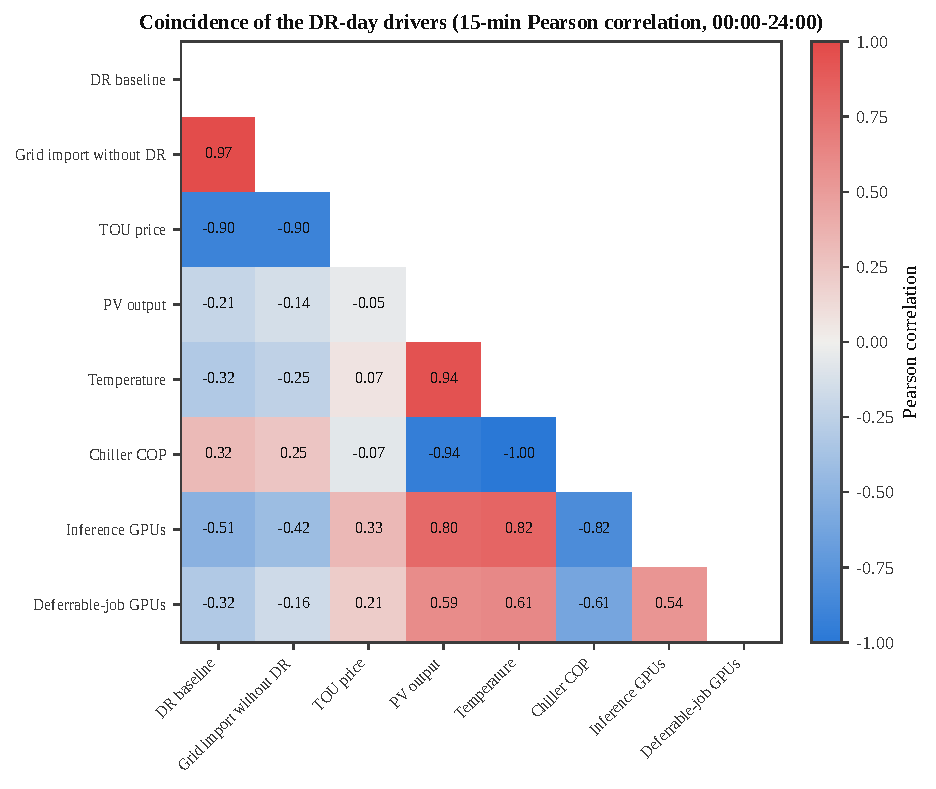
\includegraphics[width=\columnwidth]{fig17_drivers_correlation.pdf}
\caption{Pearson correlation of the DR-day drivers (15-min values). Inference load, temperature and PV peak together in
the afternoon ($r\approx0.8$); the baseline is strongly anti-correlated with the TOU price ($r=-0.90$) because the
storage discharges in the peak-price hours in normal operation.}
\label{fig:drivers}
\end{figure}

\begin{table*}[!t]
\caption{Equipment and energy-system parameters.}
\label{tab:A-equipment}
\centering\footnotesize
\begin{tabularx}{\textwidth}{@{}>{\raggedright\arraybackslash}p{0.25\textwidth}X>{\raggedright\arraybackslash}p{0.17\textwidth}@{}}
\toprule
Parameter & Value & Tag / source\\
\midrule
GPUs, node power, idle share & 16,000 H100-class GPUs; 8.4~kW per 8-GPU node (measured maximum); idle 25\% & [A] / [S]~\cite{latif2024} / [A]\\
Other IT power, auxiliary loads & 0.6~MW storage and network; $a^{\mathrm{aux}}=0.05$; 0.3~MW lighting and offices & [A]\\
Heat and cooling & $\theta=1$~MW$_{\mathrm{th}}$/MW; envelope load 0.3~MW$_{\mathrm{th}}$; chillers 30~MW$_{\mathrm{th}}$ & [A]\\
Chiller COP & $6.0-0.12(T-25)$ limited to 3--7; 4.41--5.61 on the DR day; liquid cooling $15-0.25(T-25)$ & [A]\\
BESS & 6~MW / 12~MWh, SOC 10--95\%, initial 50\%, $\eta_{\mathrm c}=\eta_{\mathrm d}=0.95$, degradation 60~CNY/MWh & [A], cost after~\cite{xu2018}\\
TES (chilled water) & 10~MWh$_{\mathrm{th}}$ (minimum 1), 4~MW$_{\mathrm{th}}$, $\eta=0.98$, loss 0.5\%/h & [A]\\
Gas engine and absorption chiller & 3~MW, $\eta_{\mathrm e}=0.38$, $\eta_{\mathrm h}=0.45$, ramp 1.5~MW/15~min; COP 0.75, 2.7~MW$_{\mathrm{th}}$ & [A]\\
PV & 8~MWp; PVWatts v5: temperature coefficient $-0.37\%$/$^\circ$C, system losses 14\% & [S]~\cite{dobos2014}\\
Connection limit & $\gamma=1.10$ of the typical-day peak $\Rightarrow16.03$~MW (sensitivity 1.0--1.3); minimum import 1.5~MW & [A]\\
Thermal inertia (optional) & 2~MWh$_{\mathrm{th}}$/K; $+3$~K rise and $-2$~K pre-cooling allowed & [A], ASHRAE A1~\cite{ashrae2021}\\
Waste-heat recovery (optional) & Heat pump 3~MW$_{\mathrm{el}}$, COP 3.5 (30 to 65~$^\circ$C); tank 0/20/40~MWh$_{\mathrm{th}}$, loss 0.5\%/h; boiler efficiency 0.9; demand $0.3\max(18-T,0)$~MW$_{\mathrm{th}}$ & [A] / [S]~\cite{meta2018odense}\\
Offshore wind (optional) & 0--40~MW; IEA 15-MW turbine (cut-in 3, rated 10.59, cut-out 25~m/s); farm efficiency 0.9; forecast error 15\% RMS, lag-1 correlation 0.97 & [S]~\cite{gaertner2020} / [A]\\
\bottomrule
\end{tabularx}
\end{table*}

\begin{table*}[!t]
\caption{Computing, market and policy parameters.}
\label{tab:A-market}
\centering\footnotesize
\begin{tabularx}{\textwidth}{@{}>{\raggedright\arraybackslash}p{0.25\textwidth}X>{\raggedright\arraybackslash}p{0.17\textwidth}@{}}
\toprule
Parameter & Value & Tag / source\\
\midrule
Workload composition & Inference $\approx$25\% of the GPUs (Azure shape), training/batch $\approx$40\% (PAI shape), of which 75\% deferrable (C1/C2/C3) & [A] / [D]\\
Inference dynamic-power factor & 0.65 & [A], after~\cite{patel2024}\\
Lag bounds & 0.5 / 1.5 / 3~h (Flex 1--3) & [A], after~\cite{colangelo2025}\\
Delay cost, overdue penalty & 0.5 and 1000~CNY per GPU$\cdot$h and hour & [A]\\
Terminal values & Backlog 0.67~CNY/GPU$\cdot$h; BESS 500~CNY/MWh; TES 100~CNY/MWh$_{\mathrm{th}}$ & computed\\
GPU power capping (optional) & One level $(0.30,0.12)$; three levels $(0.15,0.03)$, $(0.30,0.12)$, $(0.45,0.30)$; events only & [A], after~\cite{acun2026,patel2024}\\
Pause overhead (optional) & $o_c$ = 6~min (1-min checkpoint + 5-min restart) or 25~min & [A], after~\cite{wan2025,wang2023gemini}\\
TOU tariff & Jiangsu 2025 summer: peak 14--22~h ($\times$1.8), valley 0--6 and 11--13~h ($\times$0.35) & [S]\\
DR payment & 3~CNY/kWh (day-ahead), 4.2 (E3, 3~h notice), 4.8 (E3 uncertain, 1~h notice); 1--3 in sensitivity & [S]~\cite{jiangsu2024dr}\\
Validity and payment cap & Mean reduction $\ge$80\% of the commitment (+0.1~MW planning margin); payment $\le$120\% & [S]~\cite{jiangsu2024dr}\\
Shortfall coefficient & $\kappa=1$ (0.5--2) & [A]\\
Rebound charge & 0 and 3~CNY/kW per event (0--6), 2-h window & [A] (policy parameter)\\
Gas price & 3.6~CNY/Nm$^3$, lower heating value 9.89~kWh/Nm$^3$ & [A]\\
Day-ahead risk settings & SP; $\ell_1$ DRO $\delta$ = 0.1/0.2/0.4/0.8/1.2; RO ($\delta=2$); CVaR$_{0.8}$; mean--CVaR$_{0.9}$ ($w=0.5$); 10 scenarios & --\\
PUE cap (optional) & 1.30 / 1.25 / 1.20 & [S]~\cite{ndrc2024dc}\\
Green share (optional) & 60 / 80 / 90\%; green premium 30~CNY/MWh & [S]~\cite{ndrc2024dc} / [A]\\
Emission factors & Grid 0.5617~tCO$_2$/MWh; natural gas 56.1~t/TJ & [S]~\cite{mee2024ef} / IPCC 2006\\
Split of IR-R / IR-O; tuned split & $\alpha=0.41$; $\alpha^*$ back-tested over 0.2--1.0 & computed\\
\bottomrule
\end{tabularx}
\end{table*}



\begin{figure*}[!t]
\centering
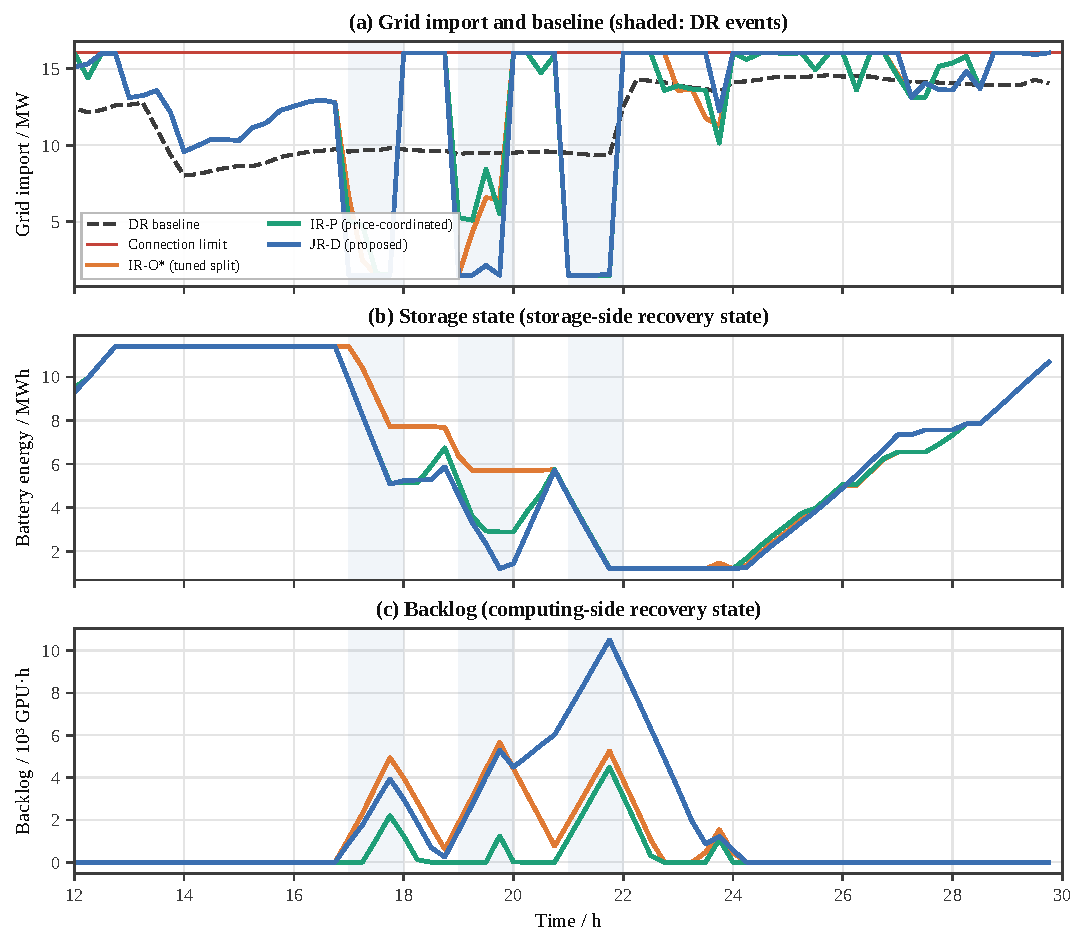
\includegraphics[width=0.82\textwidth]{fig03_timeseries_DAcommit_crb0.pdf}
\caption{Case-day time series (rule setting, coupled commitment): (a) grid import and baseline, (b) BESS energy and
(c) total backlog of JR-D, IR-O* and IR-P.}
\label{fig:ts}
\end{figure*}

\begin{figure*}[!t]
\centering
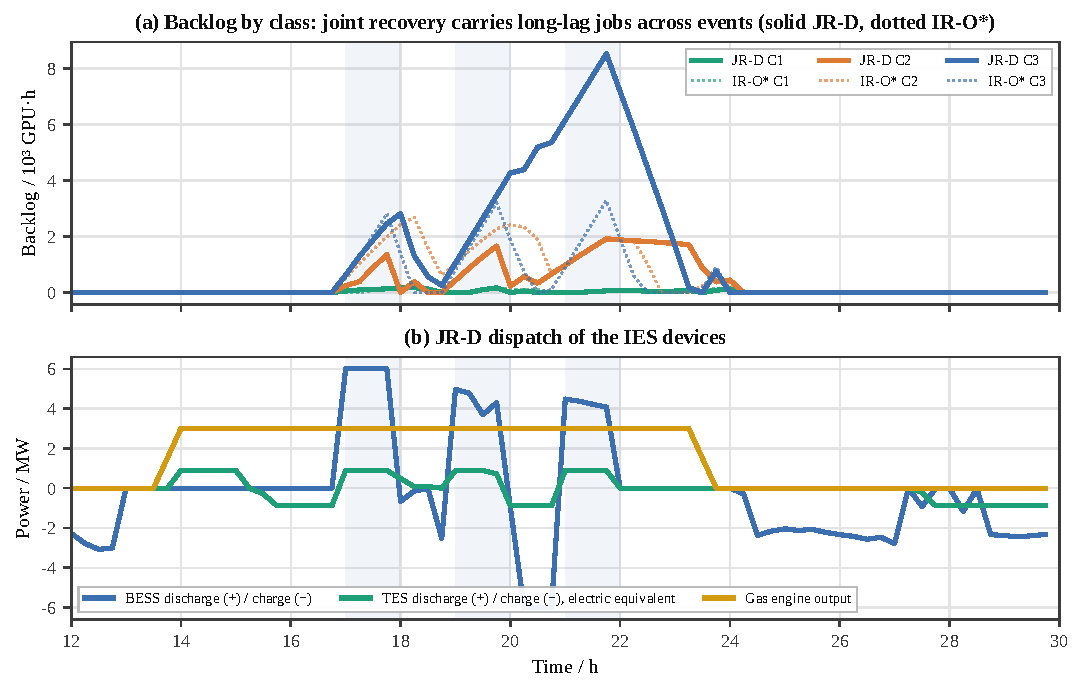
\includegraphics[width=0.82\textwidth]{fig04_backlog_ies_DAcommit_crb0.pdf}
\caption{Case-day backlog by class (solid: JR-D, dotted: IR-O*) and IES dispatch of JR-D (rule setting, coupled
commitment). Joint recovery carries the long-lag class C3 across the events.}
\label{fig:tsbacklog}
\end{figure*}
